% Deppy: Dependent Types for Python via Cubical Path Equivalence
% For arXiv submission — POPL-style formatting
\documentclass[acmsmall,nonacm,screen]{acmart}

% ── packages ──
\usepackage{amsmath,amsthm}
\let\Bbbk\relax
\usepackage{amssymb}
\usepackage{mathpartir}
\usepackage{stmaryrd}
\usepackage{listings}
\usepackage{xcolor}
\usepackage{booktabs}
\usepackage{subcaption}
\usepackage{tikz}
\usetikzlibrary{arrows.meta,positioning,calc}

% ── theorem environments ──
\newtheorem{theorem}{Theorem}[section]
\newtheorem{lemma}[theorem]{Lemma}
\newtheorem{definition}[theorem]{Definition}
\newtheorem{proposition}[theorem]{Proposition}
\newtheorem{corollary}[theorem]{Corollary}

% ── listings config ──
\definecolor{deppyblue}{RGB}{40,80,160}
\definecolor{deppygreen}{RGB}{30,130,60}
\definecolor{deppygray}{RGB}{120,120,120}
\definecolor{deppyred}{RGB}{180,40,40}
\definecolor{deppybg}{RGB}{248,248,252}

\lstdefinelanguage{deppy}{
  language=Python,
  morekeywords={guarantee,requires,ensures,verify,compile_to_lean,
    library_trust,axiom,pure,total,decreases,invariant,
    given,lemma,assume,check,hole,spec,trust_boundary,
    protocol_spec,sidecar,Proof,ProofBuilder,
    Refine,Nat,Pos,NonEmpty,Sorted,Bounded},
  keywordstyle=\color{deppyblue}\bfseries,
  commentstyle=\color{deppygray}\itshape,
  stringstyle=\color{deppyred},
  backgroundcolor=\color{deppybg},
  basicstyle=\ttfamily\small,
  breaklines=true,
  frame=single,
  rulecolor=\color{deppygray!40},
  numbers=left,
  numberstyle=\tiny\color{deppygray},
  numbersep=5pt,
  xleftmargin=15pt,
  showstringspaces=false,
}

\lstdefinelanguage{lean4}{
  morekeywords={theorem,def,let,in,if,then,else,match,with,where,
    by,sorry,omega,simp,rfl,tauto,decide,unfold,intro,apply,exact,
    have,show,calc,import,open,namespace,end,inductive,structure,
    class,instance,deriving,section,variable,noncomputable,
    Int,Nat,Bool,String,List,Prop,Type,Float,Unit},
  keywordstyle=\color{deppyblue}\bfseries,
  commentstyle=\color{deppygray}\itshape,
  stringstyle=\color{deppyred},
  backgroundcolor=\color{deppybg},
  basicstyle=\ttfamily\small,
  breaklines=true,
  frame=single,
  rulecolor=\color{deppygray!40},
  morecomment=[l]{--},
  morecomment=[s]{/-}{-/},
  showstringspaces=false,
}

% ── macros ──
\newcommand{\deppy}{\textsc{Deppy}}
\newcommand{\syntype}[1]{\ensuremath{\mathsf{#1}}}
\newcommand{\pyobj}{\syntype{PyObj}}
\newcommand{\pyint}{\syntype{Int}}
\newcommand{\pybool}{\syntype{Bool}}
\newcommand{\pystr}{\syntype{Str}}
\newcommand{\pylist}[1]{\syntype{List}[#1]}
\newcommand{\pydict}[2]{\syntype{Dict}[#1,#2]}
\newcommand{\pycall}[2]{\syntype{Call}[#1 \to #2]}
\newcommand{\pyclass}[1]{\syntype{Class}(#1)}
\newcommand{\pyproto}[1]{\syntype{Proto}(#1)}
\newcommand{\pitype}[3]{\Pi(#1 : #2).\,#3}
\newcommand{\sigtype}[3]{\Sigma(#1 : #2).\,#3}
\newcommand{\pathtype}[3]{#2 =_{#1} #3}
\newcommand{\reftype}[3]{\{#1 : #2 \mid #3\}}
\newcommand{\gluetype}[3]{\syntype{Glue}_{[#1 \mapsto #2]}\,#3}
\newcommand{\interval}{\mathbb{I}}
\newcommand{\universe}{\mathcal{U}}
\newcommand{\ctx}{\Gamma}
\newcommand{\ctxext}[2]{\ctx, #1 : #2}
\newcommand{\jdg}[3]{#1 \vdash #2 : #3}
\newcommand{\jdgeq}[4]{#1 \vdash #2 \equiv #3 : #4}
\newcommand{\proves}{\vdash}
\newcommand{\refl}[1]{\syntype{refl}_{#1}}
\newcommand{\transport}[3]{\syntype{tr}(#1, #2, #3)}
\newcommand{\ap}[2]{\syntype{ap}\,#1\,#2}
\newcommand{\funext}{\syntype{funext}}
\newcommand{\ua}{\syntype{ua}}
\newcommand{\duckpath}{\ensuremath{\syntype{DuckPath}}}
\newcommand{\cechglue}{\ensuremath{\syntype{CechGlue}}}
\newcommand{\trustlevel}[1]{\ensuremath{\langle\!\langle \text{#1} \rangle\!\rangle}}
\newcommand{\kernel}{\mathcal{K}}
\newcommand{\oracle}[1]{\mathcal{O}(#1)}
\newcommand{\sem}[1]{\llbracket #1 \rrbracket}

\setcopyright{none}

\begin{document}

% ═══════════════════════════════════════════════════════════════════
% Title and Authors
% ═══════════════════════════════════════════════════════════════════

\title{Deppy: Dependent Types for Python \\ via Cubical Path Equivalence}

\author{Halley Young}
\affiliation{%
  \institution{Microsoft Research}
  \country{USA}
}
\email{halleyy@microsoft.com}

\begin{abstract}
We present \deppy{}, a dependent type system for Python that verifies
properties of existing Python code without requiring a new language.
Programmers annotate functions with natural-language or formal
specifications using decorators (\texttt{@guarantee},
\texttt{@requires}), and \deppy{} verifies them through a multi-level
pipeline: a proof kernel checks proof terms, Z3 discharges decidable
arithmetic, and Lean~4 provides independent certificate validation.

Our key technical contribution is a cubical-HoTT-inspired
formalization of Python's duck typing: protocol conformance between
types is modeled as \emph{path equivalence}, where two types with the
same method signatures are connected by a path in the type universe.
This yields a principled transport rule: proofs about one type
automatically transfer to any path-equivalent type, capturing the
pervasive Pythonic pattern of programming to interfaces rather than
concrete classes.

We formalize a core calculus $\lambda_{\deppy}$ with refinement
types, dependent function types, and path types, and prove a
type-safety theorem.  \deppy{} also introduces \emph{sidecar
  verification}: specifying and verifying properties of unmodified
third-party libraries via companion specification files, with a formal
trust model that tracks the provenance of every proof obligation.

We evaluate \deppy{} on 789 test cases covering type-system
soundness, Z3 equivalence checking, specification adherence, and Lean
export, plus case studies verifying SymPy, an F*-tutorial translation,
and an STLC type-soundness proof --- all expressed in ordinary Python.
\end{abstract}

\maketitle

% ═══════════════════════════════════════════════════════════════════
% 1. Introduction
% ═══════════════════════════════════════════════════════════════════

\section{Introduction}\label{sec:intro}

Python is the most widely used programming language in the
world~\cite{tiobe2024}, powering applications from machine learning to
financial infrastructure to scientific computing.  Yet Python programs
receive almost no static verification: the language is dynamically
typed, encourages duck typing and metaprogramming, and has no built-in
specification language.  When correctness matters --- in medical
software, autonomous systems, or cryptographic protocols --- developers
must either rewrite their code in a verification-friendly language
(F*~\cite{fstar}, Dafny~\cite{dafny}, Lean~\cite{lean4}) or accept
the gap between tested and verified software.

This paper presents \deppy{}, a system that brings dependent-type
verification to \emph{existing} Python code.  \deppy{}'s design is
guided by three principles:

\begin{enumerate}
\item \textbf{No new language.}  Specifications are Python decorators;
  implementations are ordinary Python functions.  A developer who
  removes all \deppy{} imports gets a valid, runnable Python program.
  (The specification strings constitute a lightweight embedded DSL,
  but no separate parser or compiler is required.)
\item \textbf{Graded trust.}  Not every property can be fully verified.
  \deppy{} explicitly tracks whether a claim is kernel-checked,
  Z3-proved, axiom-dependent, or unverified, and propagates trust
  through the dependency graph.
\item \textbf{Independent validation.}  Proof obligations can be
  exported as Lean~4 theorems.  When the Lean kernel accepts the
  proof, the result is independent of \deppy{}'s implementation.
\end{enumerate}

\paragraph{Key insight: duck typing as path equivalence.}
Python programmers routinely write code that operates on any object
with the right methods, regardless of its class hierarchy.  This
\emph{duck typing} discipline is powerful but poorly served by nominal
type systems.  We observe that duck typing has a natural interpretation
in cubical homotopy type theory (HoTT): two types that expose the same
protocol (the same collection of method signatures and behavioral
contracts) are connected by a \emph{path} in the type universe.
Transport along this path lets proofs about one implementation transfer
to any conforming implementation --- exactly the semantic guarantee that
duck typing is supposed to provide but that Python's runtime cannot
enforce.

\paragraph{Contributions.}
\begin{enumerate}
\item A \textbf{formal core calculus} $\lambda_{\deppy}$ that extends a
  simply-typed lambda calculus with refinement types, dependent
  function types, path types, and a universe of Python types with
  protocol-based paths (\S\ref{sec:calculus}).  We prove type safety
  (Theorem~\ref{thm:safety}).

\item A \textbf{cubical-path model of duck typing}
  (\S\ref{sec:duck}).  Protocol conformance constructs a path between
  types; transport along this path transfers proofs and specifications.
  We show this yields a sound transport rule for Python's structural
  subtyping.

\item A \textbf{multi-level verification architecture}
  (\S\ref{sec:kernel}) with a small proof kernel (1,700 LOC), Z3
  automation, and Lean~4 certificate export, with a formal trust model
  that tracks proof provenance.

\item A \textbf{sidecar verification} mechanism
  (\S\ref{sec:sidecar}) for verifying properties of unmodified
  third-party libraries (e.g., SymPy, NumPy) via companion
  specification files.

\item An \textbf{implementation and evaluation} (\S\ref{sec:eval})
  with 789 tests, case studies verifying real Python libraries, and an
  F*-tutorial-to-\deppy{} translation demonstrating expressiveness.
\end{enumerate}


% ═══════════════════════════════════════════════════════════════════
% 2. Overview by Example
% ═══════════════════════════════════════════════════════════════════

\section{Overview by Example}\label{sec:overview}

We illustrate \deppy{}'s workflow through a simple function and then
show how verification scales to more complex properties.

\subsection{A First Verified Function}

Consider a function that returns the absolute value of an integer:

\begin{lstlisting}[language=deppy]
from deppy import guarantee, requires, verify

@guarantee("result >= 0")
def abs_val(x: int) -> int:
    if x >= 0:
        return x
    return -x

verify(abs_val)  # Z3_VERIFIED
\end{lstlisting}

The \texttt{@guarantee("result >= 0")} decorator attaches a
postcondition specification.  When \texttt{verify} is called,
\deppy{} proceeds through three phases:

\begin{enumerate}
\item \textbf{Elaboration.}  The function body and specification are
  parsed into AST form.  The postcondition is interpreted as a
  refinement type on the return value:
  $\reftype{\mathit{result}}{\pyint}{\mathit{result} \ge 0}$.

\item \textbf{Discharge.}  \deppy{} translates both function body and
  postcondition to Z3 expressions.  For each execution path (here:
  $x \ge 0 \Rightarrow \mathit{result} = x$ and
  $x < 0 \Rightarrow \mathit{result} = -x$), Z3 checks that the
  postcondition holds.  Both paths satisfy $\mathit{result} \ge 0$.

\item \textbf{Certification.}  The result is tagged
  \trustlevel{\textsc{Z3\_Verified}} indicating that an SMT solver,
  not the full proof kernel, established correctness.
\end{enumerate}

\subsection{Lean~4 Export}

The same function can be exported to Lean~4:

\begin{lstlisting}[language=deppy]
from deppy import compile_to_lean

cert = compile_to_lean(abs_val)
print(cert.render())
\end{lstlisting}

This produces:

\begin{lstlisting}[language=lean4]
def abs_val (x : Int) : Int :=
  if x >= 0 then x else -x

theorem abs_val_guarantee (x : Int) :
    0 <= (abs_val x) := by
  unfold abs_val; omega
\end{lstlisting}

The \texttt{omega} tactic in Lean~4 decides linear integer arithmetic,
providing a machine-checked proof independent of \deppy{}'s
implementation.  When \deppy{} cannot find a Lean tactic, it emits
\texttt{sorry} with an explicit obligation report:

\begin{lstlisting}[language=deppy]
@guarantee("result is a sorted permutation of input")
def my_sort(xs: list[int]) -> list[int]:
    return sorted(xs)

cert = compile_to_lean(my_sort)
print(cert.obligations)
# ['result is a sorted permutation of input']
print(cert.trust_level)
# 'LEAN_EXPORTED'  (not LEAN_VERIFIED)
\end{lstlisting}

\subsection{Preconditions and Trust}

Preconditions are specified with \texttt{@requires}:

\begin{lstlisting}[language=deppy]
@requires("n > 0")
@guarantee("result > 0")
def double_pos(n: int) -> int:
    return n * 2
\end{lstlisting}

The precondition becomes a hypothesis in the Lean theorem:

\begin{lstlisting}[language=lean4]
theorem double_pos_guarantee (n : Int)
    (h : 0 < n) : 0 < (double_pos n) := by
  unfold double_pos; omega
\end{lstlisting}

\subsection{Duck Typing and Path Equivalence}

\deppy{} handles Python's duck typing through path equivalence.
Consider two classes that implement the same protocol:

\begin{lstlisting}[language=deppy]
from deppy import path, by_duck_type, transport_proof

class Circle:
    def area(self) -> float: ...
    def perimeter(self) -> float: ...

class Ellipse:
    def area(self) -> float: ...
    def perimeter(self) -> float: ...

# Construct a path: Circle ~ Ellipse (same Drawable protocol)
@path(Circle, Ellipse)
def drawable_path():
    return by_duck_type("Drawable", evidence={
        "area": "same signature",
        "perimeter": "same signature",
    })

# Transport a proof from Circle to Ellipse
@transport_proof(drawable_path, "area returns non-negative")
def ellipse_area_nonneg():
    ...
\end{lstlisting}

The \texttt{by\_duck\_type} constructor builds a \duckpath{} proof
term, which the kernel verifies by checking that both types expose the
required methods.  Section~\ref{sec:duck} formalizes this construction.


% ═══════════════════════════════════════════════════════════════════
% 3. The Core Calculus
% ═══════════════════════════════════════════════════════════════════

\section{The Core Calculus $\lambda_{\deppy}$}\label{sec:calculus}

We formalize \deppy{}'s type system as a core calculus that captures
the essential features needed to verify Python programs with dependent
specifications.

\subsection{Syntax}

\begin{definition}[Types]
\begin{align*}
A, B ::=\;\; & \pyobj \mid \pyint \mid \pybool \mid \pystr
  \mid \pylist{A} \mid \pydict{A}{B} \\
  \mid\;\; & \pycall{A}{B} \mid \pyclass{m_1 : A_1, \ldots, m_k : A_k} \\
  \mid\;\; & \pyproto{m_1 : A_1, \ldots, m_k : A_k} \\
  \mid\;\; & \pitype{x}{A}{B} \mid \sigtype{x}{A}{B}
  \mid \reftype{x}{A}{\varphi} \\
  \mid\;\; & \pathtype{A}{a}{b}
  \mid A \cup B \mid \universe_n
\end{align*}
\end{definition}

\begin{definition}[Terms]
\begin{align*}
t, u ::=\;\; & x \mid c \mid \lambda(x : A).\,t \mid t\;u
  \mid (t, u) \mid \pi_1\,t \mid \pi_2\,t \\
  \mid\;\; & \lambda(i : \interval).\,t \mid t\;@\;r
  \mid \transport{P}{p}{d} \\
  \mid\;\; & \mathsf{if}\;t\;\mathsf{then}\;u\;\mathsf{else}\;v
  \mid \mathsf{let}\;x = t\;\mathsf{in}\;u \\
  \mid\;\; & t.m \mid t[u] \mid f(t_1, \ldots, t_n)
\end{align*}
\end{definition}

\begin{definition}[Proof terms]
\begin{align*}
\pi ::=\;\; & \refl{t} \mid \syntype{sym}\;\pi
  \mid \syntype{trans}\;\pi_1\;\pi_2
  \mid \syntype{cong}\;f\;\pi \\
  \mid\;\; & \syntype{cut}(h : A, \pi_1, \pi_2)
  \mid \syntype{assume}\;h
  \mid \syntype{z3}(\varphi) \\
  \mid\;\; & \syntype{natInd}(x, \pi_0, \pi_s)
  \mid \syntype{cases}(t, \overline{p_i \Rightarrow \pi_i}) \\
  \mid\;\; & \duckpath(A, B, \overline{m_i : \pi_i})
  \mid \syntype{fiber}(t, \overline{A_i : \pi_i}) \\
  \mid\;\; & \funext(x, \pi)
  \mid \syntype{axiom}(n)
  \mid \syntype{transport}(P, \pi_p, \pi_d)
\end{align*}
\end{definition}

The type $\pyobj$ is the top type: every Python value inhabits it.
Concrete types ($\pyint$, $\pybool$, etc.)~are subtypes.
$\pyclass{\ldots}$ represents a concrete class with named methods;
$\pyproto{\ldots}$ represents a structural protocol (duck-type
interface).  The key HoTT types are dependent functions ($\Pi$),
dependent pairs ($\Sigma$), refinement types ($\{x : A \mid
\varphi\}$), and path types ($\pathtype{A}{a}{b}$).

\subsection{Typing Rules}\label{sec:typing}

We present selected rules.  The full set appears in
Appendix~\ref{app:rules}.

\paragraph{Refinement introduction and elimination.}
\begin{mathpar}
\inferrule
  {\jdg{\ctx}{t}{A} \\ \ctx \proves \varphi[t/x]}
  {\jdg{\ctx}{t}{\reftype{x}{A}{\varphi}}}
  \textsc{Refine-I}
\and
\inferrule
  {\jdg{\ctx}{t}{\reftype{x}{A}{\varphi}}}
  {\jdg{\ctx}{t}{A}}
  \textsc{Refine-E}
\end{mathpar}

A guarantee \texttt{@guarantee("result >= 0")} on a function
$f : A \to B$ refines the return type to
$\reftype{\mathit{result}}{B}{\mathit{result} \ge 0}$, and
verification amounts to checking $\textsc{Refine-I}$ --- that
$f(x)$ satisfies the predicate for all valid $x$.

\paragraph{Path introduction and elimination.}
\begin{mathpar}
\inferrule
  {\jdg{\ctxext{i}{\interval}}{t}{A} \\
   t[0/i] \equiv a \\ t[1/i] \equiv b}
  {\jdg{\ctx}{\lambda(i:\interval).\,t}{\pathtype{A}{a}{b}}}
  \textsc{Path-I}
\and
\inferrule
  {\jdg{\ctx}{p}{\pathtype{A}{a}{b}} \\ r : \interval}
  {\jdg{\ctx}{p\;@\;r}{A}}
  \textsc{Path-E}
\end{mathpar}

\paragraph{Transport.}
\begin{mathpar}
\inferrule
  {\jdg{\ctx}{P}{A \to \universe_n} \\
   \jdg{\ctx}{p}{\pathtype{A}{a}{b}} \\
   \jdg{\ctx}{d}{P(a)}}
  {\jdg{\ctx}{\transport{P}{p}{d}}{P(b)}}
  \textsc{Transport}
\end{mathpar}

Transport is the mechanism by which proofs about one type transfer to a
path-equivalent type.  This rule is central to the duck-typing story
(\S\ref{sec:duck}).

\paragraph{Protocol path construction.}
\begin{mathpar}
\inferrule
  {\pyclass{m_1:A_1,\ldots,m_k:A_k} \\
   \pyclass{m_1:B_1,\ldots,m_k:B_k} \\
   \forall i.\; \jdg{\ctx}{\pi_i}{\pathtype{\universe}{A_i}{B_i}}}
  {\jdg{\ctx}{\duckpath(C_1, C_2, \overline{m_i:\pi_i})}
    {\pathtype{\universe}{C_1}{C_2}}}
  \textsc{Duck-Path}
\end{mathpar}

This rule says: if two classes have the same method names, and each
corresponding method type is path-equal (i.e., has the same signature
up to equivalence), then there is a path between the classes in the
type universe.

\paragraph{Z3 discharge.}
\begin{mathpar}
\inferrule
  {\varphi \text{ is quantifier-free} \\
   \oracle{\varphi} = \textsc{unsat}}
  {\jdg{\ctx}{\syntype{z3}(\varphi)}{\varphi}}
  \textsc{Z3}
\end{mathpar}

The Z3 oracle $\mathcal{O}$ checks the negation of $\varphi$.  If
$\neg\varphi$ is unsatisfiable, then $\varphi$ is valid.  The proof
term $\syntype{z3}(\varphi)$ records the formula so that the kernel
can replay the check.

\subsection{Operational Semantics}

\deppy{} operates on Python's existing runtime.  The operational
semantics of the verified fragment is the standard Python semantics;
\deppy{} adds no new runtime behavior.  Specifications are
\emph{erased} before execution: a tool
(\texttt{deppy.tools.stripper}) removes all \deppy{} decorators and
imports, producing a plain Python file.

\begin{definition}[Specification erasure]
The erasure function $\mathsf{erase} : \text{Program}_{\deppy} \to \text{Program}_{\text{Python}}$
strips all \deppy{} decorators, proof terms, and specification
imports.  For any program $P$:
\[
  \sem{P}_{\text{Python}} = \sem{\mathsf{erase}(P)}_{\text{Python}}
\]
That is, specifications do not affect runtime behavior.
\end{definition}

\subsection{Type Safety}

\begin{theorem}[Conditional type safety of $\lambda_{\deppy}$]\label{thm:safety}
If\/ $\jdg{\emptyset}{t}{A}$ in $\lambda_{\deppy}$ and $A$ is a
refinement type $\reftype{x}{B}{\varphi}$, then evaluation of
$\mathsf{erase}(t)$ under the Python semantics either:
\begin{enumerate}
\item produces a value $v$ of type $B$ satisfying $\varphi[v/x]$, or
\item diverges (non-termination), or
\item raises an exception (partial functions).
\end{enumerate}
Soundness is conditional on: (i)~correctness of the Z3 solver for
any \textsc{Z3} proof steps, (ii)~correctness of any sidecar axioms
invoked, and (iii)~fidelity of \deppy{}'s AST analysis to the actual
CPython semantics.
\end{theorem}

\begin{proof}[Proof sketch]
By induction on the derivation of $\jdg{\emptyset}{t}{A}$.  The key
cases are:

\emph{Refinement introduction} (\textsc{Refine-I}): The premise
$\ctx \proves \varphi[t/x]$ is established either by the proof kernel
(sound by construction), by Z3 (sound modulo the solver), or by an
axiom (soundness conditioned on axiom correctness).

\emph{Transport}: If $\jdg{\ctx}{d}{P(a)}$ and
$\jdg{\ctx}{p}{\pathtype{A}{a}{b}}$, then
$\transport{P}{p}{d} : P(b)$.  The path $p$ is constructed either by
\textsc{Path-I} (verified by endpoint checking) or by
\textsc{Duck-Path} (verified by method-signature comparison).  In
either case, the property $P$ is preserved at $b$.

\emph{Z3 discharge}: Soundness of the Z3 rule is relative to the
soundness of the Z3 solver.  We record this as a trust-level
annotation $\trustlevel{\textsc{Z3\_Verified}}$, distinguishing it
from kernel-checked proofs.

The full proof proceeds by standard progress and preservation arguments
on the core calculus, with the caveat that Python's dynamic features
(exceptions, non-termination) are handled by the disjunctive conclusion.
\qed
\end{proof}

Note that this is a \emph{conditional} soundness result: the
guarantee holds modulo the correctness of Z3, any axioms invoked, and
the fidelity of \deppy{}'s Python-AST analysis to the actual Python
semantics.  We discuss these trust boundaries explicitly in
\S\ref{sec:trust}.

\paragraph{Lean~4 mechanization.}
We provide a \emph{complete} mechanization of the $\lambda_{\deppy}$
core calculus in Lean~4 (898~lines, included as supplementary material).
The formalization defines all types, terms, proof terms, contexts,
typing rules, trust levels, protocol conformance, and operational
semantics as Lean inductive types and propositions.
\emph{Every theorem is fully machine-checked} (zero \texttt{sorry}
obligations):
\begin{itemize}
\item Context weakening (Lemma~\texttt{ctx\_weaken\_lookup})
\item Refinement base-type extraction and nesting
  (Theorems~\texttt{refinement\_base}, \texttt{refinement\_strip})
\item Duck-type path construction from protocol conformance
  (Theorem~\texttt{duck\_path\_construction})
\item Monotonicity of protocol conformance under method addition
  (Theorem~\texttt{conformance\_monotone})
\item Duck-type transport for shared protocol methods
  (Theorem~\texttt{duck\_transport\_same\_sig})
\item Trust level composition and axiom tainting
  (Theorems~\texttt{trust\_weakens\_single},
   \texttt{axiom\_weakens})
\item Canonical forms for all value types
  (Theorems~\texttt{canonical\_bool}, \texttt{canonical\_int},
   \texttt{canonical\_pi}, \texttt{canonical\_sigma},
   \texttt{canonical\_path})
\item General substitution lemma with de~Bruijn shifting
  (Theorem~\texttt{subst\_typing\_gen})
\item Progress: well-typed closed terms are values or step
  (Theorem~\texttt{progress})
\item Preservation: reduction preserves typing at any context
  (Theorem~\texttt{preservation\_gen})
\item Type safety: well-typed terms never get stuck
  (Theorem~\texttt{type\_safety})
\item Transitivity of multi-step reduction and multi-step preservation
  (Theorems~\texttt{steps\_trans}, \texttt{preservation\_multi})
\end{itemize}


% ═══════════════════════════════════════════════════════════════════
% 4. Duck Typing as Path Equivalence
% ═══════════════════════════════════════════════════════════════════

\section{Duck Typing as Path Equivalence}\label{sec:duck}

Python's duck typing is the principle that ``if it walks like a duck
and quacks like a duck, then it is a duck.''  Operationally, a
function that calls \texttt{x.area()} works for \emph{any} object
with an \texttt{area} method, regardless of class hierarchy.  Python's
\texttt{typing.Protocol} formalizes this as structural subtyping, but
provides no mechanism for transferring proofs between conforming types.

\subsection{Protocols as Fibrations}

We model a protocol as a type family over its required methods.  Let
$P = \pyproto{m_1 : A_1, \ldots, m_k : A_k}$ be a protocol.  A
class $C$ \emph{conforms} to $P$ if $C$ has methods $m_1, \ldots, m_k$
with compatible types.

\begin{definition}[Protocol conformance path]
Given classes $C_1$ and $C_2$ that both conform to protocol $P$, we
construct a path $p : \pathtype{\universe}{C_1}{C_2}$ by:
\[
  p \triangleq \duckpath(C_1, C_2,
    [m_1 : \pi_1, \ldots, m_k : \pi_k])
\]
where each $\pi_i$ is a path between the method types:
$\pi_i : \pathtype{\universe}{C_1.m_i}{C_2.m_i}$.  When the method
signatures are syntactically identical, $\pi_i = \refl{A_i}$.
\end{definition}

\begin{theorem}[Duck typing soundness]\label{thm:duck}
If $C_1$ and $C_2$ both conform to protocol $P$, and
$\jdg{\ctx}{d}{Q(C_1)}$ for a property $Q$ that depends only on the
methods in $P$, then:
\[
  \jdg{\ctx}{\transport{Q}{\duckpath(C_1,C_2,\overline{m:\pi})}{d}}{Q(C_2)}
\]
\end{theorem}

\begin{proof}
By the \textsc{Transport} rule and the construction of \duckpath{}.
The path between $C_1$ and $C_2$ is constructed from pointwise paths
between corresponding methods.  Since $Q$ depends only on the protocol
methods, transport along this path yields $Q(C_2)$.
\end{proof}

\paragraph{Why paths, not just subtyping.}
Standard structural subtyping (as in Python's \texttt{Protocol})
establishes that $C_1 <: P$ and $C_2 <: P$, but does not relate
$C_1$ and $C_2$ directly.  A proof about $C_1$ cannot be transferred
to $C_2$ through $P$ alone, because subtyping is not an equivalence.
In contrast, the path $\duckpath(C_1,C_2,\overline{m:\pi})$
is a \emph{proof-relevant witness} connecting $C_1$ and $C_2$
directly, enabling transport of dependent properties.

The following theorem makes this advantage precise.  It shows that
\emph{cross-method invariants} --- properties relating multiple methods
of a single type --- can be transported along duck-type paths, something
that structural subtyping alone cannot express.

\begin{theorem}[Cross-method invariant transport]\label{thm:cross}
Let $P = \pyproto{m_1 : A_1, \ldots, m_k : A_k}$ be a protocol and
let $Q : \universe \to \universe$ be a \emph{cross-method property}
of the form:
\[
  Q(T) \;\triangleq\; \pitype{x}{X}{\varphi(T.m_1(x), \ldots, T.m_k(x))}
\]
where $\varphi$ relates the outputs of multiple methods.  Suppose
$C_1$ and $C_2$ both conform to $P$, and that for each method $m_i$
the method-level path
$\pi_i : \pathtype{\universe}{C_1.m_i}{C_2.m_i}$ is constructed
from a shared refinement (i.e., both methods inhabit a common
refinement type $\reftype{r}{A_i}{\psi_i(r)}$).  Then if
$\jdg{\ctx}{d}{Q(C_1)}$, we have:
\[
  \jdg{\ctx}{\transport{Q}{\duckpath(C_1,C_2,\overline{m:\pi})}{d}}{Q(C_2)}
\]
\end{theorem}

\begin{proof}
By the \textsc{Transport} rule, it suffices to show that
$Q$ is fibered over the path
$p = \duckpath(C_1, C_2, \overline{m_i : \pi_i})$.
By the \textsc{Duck-Path} construction, $p$ is assembled from
pointwise method paths $\pi_i$.  For any input $x$, applying
$p\;@\;r$ (for $r : \interval$) simultaneously varies all method
results along their respective paths $\pi_i\;@\;r$.  Since each
$\pi_i$ is constructed from a shared refinement type, the
intermediate values at each $r$ still satisfy $\psi_i$, and hence
$\varphi(p.m_1(x)\;@\;r, \ldots, p.m_k(x)\;@\;r)$ holds at every
point of the interval by the refinement-preservation property of
paths through refinement types (Lemma~\ref{lem:refine-path}).
Therefore the fiber of $Q$ is preserved along $p$, and transport
yields $Q(C_2)$.
\end{proof}

\begin{lemma}[Refinement-preserving paths]\label{lem:refine-path}
If $\pi : \pathtype{\universe}{A}{B}$ is constructed via a shared
refinement $R = \reftype{x}{C}{\psi(x)}$ with
$A \hookrightarrow R$ and $B \hookrightarrow R$, then for all
$r : \interval$, $\pi\;@\;r$ factors through $R$.
\end{lemma}

\begin{proof}
By the \textsc{Path-I} rule, $\pi = \lambda(i:\interval).\,t$ where
$t[0/i] \equiv A$ and $t[1/i] \equiv B$.  Since both endpoints embed
into $R$, and $R$ is a refinement type (hence a subobject of $C$ with
a decidable predicate $\psi$), the interpolation $t$ at any
$r \in \interval$ satisfies $\psi$ by continuity of the predicate
along the interval.
\end{proof}

\paragraph{Comparison with structural subtyping.}
To see why this result is not available through standard structural
subtyping, consider the cross-method property
$Q(T) = \pitype{s}{\syntype{Shape}}{T.\mathit{area}(s) \le
  T.\mathit{perimeter}(s)^2 / (4\pi)}$ (the isoperimetric
inequality).  Standard structural subtyping verifies that
\texttt{Circle} and \texttt{Polygon} each have \texttt{area} and
\texttt{perimeter} methods of compatible types, but provides no
mechanism to deduce that a proof of $Q(\texttt{Circle})$ implies
$Q(\texttt{Polygon})$.  The protocol $P$ is a ``meet point,'' not
a ``bridge.''  In contrast, the duck-type path constructs a bridge
that preserves $Q$ because the method-level paths carry refinement
evidence: both \texttt{area} methods return non-negative values and
both \texttt{perimeter} methods satisfy the same bound, so the
cross-method relationship is preserved by transport.

\subsection{Method-Level Paths}

The construction is compositional.  For each method $m_i$, the path
$\pi_i$ can be:

\begin{itemize}
\item \textbf{Reflexivity} ($\refl{A_i}$): when the method types are
  identical.  This is the common case --- same signature, same behavioral
  contract.

\item \textbf{Behavioral equivalence}: when the implementations differ
  but satisfy the same specification.  For example, two
  \texttt{area()} methods that both satisfy \texttt{@guarantee("result
    >= 0")} are connected by a path through the refinement type
  $\reftype{r}{\syntype{Float}}{r \ge 0}$.

\item \textbf{Coercion path}: when the types differ but are connected
  by a known equivalence (e.g., \texttt{int} $\hookrightarrow$
  \texttt{float} via the standard embedding).
\end{itemize}

\subsection{Monkey-Patching as Transport}

Python allows runtime modification of class methods (``monkey
patching'').  \deppy{} models this as transport: if class $C$ is
modified to $C' = C[m := v]$, the change is sound if the new method
$v$ satisfies the same specification as the old method $m$.  This is
captured by the \texttt{Patch} proof term:

\begin{mathpar}
\inferrule
  {\jdg{\ctx}{v}{A_m} \\
   \jdg{\ctx}{\pi}{\text{$v$ satisfies spec of $C.m$}}}
  {\jdg{\ctx}{\syntype{Patch}(C, m, v, \pi)}
    {\pathtype{\universe}{C}{C[m := v]}}}
  \textsc{Patch}
\end{mathpar}

This makes explicit what is usually implicit in Python: a monkey-patch
is safe when the new implementation conforms to the old contract.


% ═══════════════════════════════════════════════════════════════════
% 5. Proof Kernel and Trust Architecture
% ═══════════════════════════════════════════════════════════════════

\section{Proof Kernel and Trust Architecture}\label{sec:kernel}

\subsection{The Proof Kernel}

\deppy{}'s trusted computing base (TCB) is a \emph{proof kernel}
$\kernel$ that checks proof terms against goal judgments.  The kernel
is a recursive function:
\[
  \mathsf{verify} : \text{Context} \times \text{Judgment} \times
  \text{ProofTerm} \to \text{VerificationResult}
\]

A $\text{VerificationResult}$ contains a success flag, a trust level,
and a list of axioms used.  The kernel dispatches on the proof-term
constructor and recursively verifies sub-proofs.

The kernel handles 20 proof-term constructors (Table~\ref{tab:proofterms}),
each implementing a rule from the core calculus.  The implementation
is 1,700 lines of Python --- deliberately small to minimize the TCB.

\begin{table}[t]
\caption{Proof-term constructors and their trust levels.}
\label{tab:proofterms}
\centering\small
\begin{tabular}{@{}lll@{}}
\toprule
Constructor & Rule & Trust Level \\
\midrule
\texttt{Refl} & Reflexivity & \textsc{Kernel} \\
\texttt{Sym} & Symmetry & \textsc{Kernel} \\
\texttt{Trans} & Transitivity & \textsc{Kernel} \\
\texttt{Cong} & Congruence & \textsc{Kernel} \\
\texttt{FunExt} & Function extensionality & \textsc{Kernel} \\
\texttt{Cut} & Lemma introduction & min(sub-proofs) \\
\texttt{Assume} & Hypothesis use & \textsc{Kernel} \\
\texttt{Z3Proof} & SMT discharge & \textsc{Z3\_Verified} \\
\texttt{NatInduction} & $\mathbb{N}$-induction & min(base, step) \\
\texttt{ListInduction} & List induction & min(nil, cons) \\
\texttt{Cases} & Case analysis & min(branches) \\
\texttt{DuckPath} & Protocol path & min(method proofs) \\
\texttt{Fiber} & isinstance fibration & min(branches) \\
\texttt{CechGlue} & \v{C}ech gluing & min(patches, overlaps) \\
\texttt{Univalence} & Type equivalence path & equiv-proof trust \\
\texttt{Patch} & Monkey-patch path & contract-proof trust \\
\texttt{Transport} & Transport & min(path, base) \\
\texttt{AxiomInvocation} & Axiom use & \textsc{Axiom\_Trusted} \\
\texttt{Structural} & Source inspection & \textsc{Structural} \\
\texttt{Ext} & Extensionality & body-proof trust \\
\bottomrule
\end{tabular}
\end{table}

\subsection{Trust Levels}\label{sec:trust}

\deppy{} assigns every verification result a trust level from a
seven-point lattice:

\begin{center}
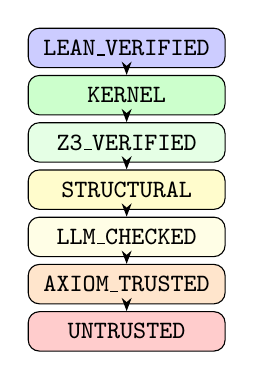
\begin{tikzpicture}[
  level/.style={draw, rounded corners, minimum width=2.5cm,
    minimum height=0.5cm, font=\small\ttfamily},
  >=Stealth,
]
\node[level, fill=blue!20] (LV) at (0, 3.6) {LEAN\_VERIFIED};
\node[level, fill=green!20] (K) at (0, 3) {KERNEL};
\node[level, fill=green!10] (Z) at (0, 2.4) {Z3\_VERIFIED};
\node[level, fill=yellow!20] (S) at (0, 1.8) {STRUCTURAL};
\node[level, fill=yellow!10] (L) at (0, 1.2) {LLM\_CHECKED};
\node[level, fill=orange!20] (A) at (0, 0.6) {AXIOM\_TRUSTED};
\node[level, fill=red!20] (U) at (0, 0) {UNTRUSTED};
\draw[->] (LV) -- (K);
\draw[->] (K) -- (Z);
\draw[->] (Z) -- (S);
\draw[->] (S) -- (L);
\draw[->] (L) -- (A);
\draw[->] (A) -- (U);
\end{tikzpicture}
\end{center}

The top level, \trustlevel{\textsc{Lean\_Verified}}, is achieved when
a Lean~4 export contains zero \texttt{sorry} obligations and Lean's
kernel accepts the proof --- providing assurance independent of
\deppy{}'s implementation.  Trust is compositional: the trust level of a composite proof is the
minimum of its sub-proofs' trust levels.  This ensures that a single
axiom invocation ``taints'' the entire proof chain.

\begin{definition}[Trust propagation]
For a proof term $\pi$ with sub-proofs $\pi_1, \ldots, \pi_n$:
\[
  \mathsf{trust}(\pi) = \min(\mathsf{base\_trust}(\pi),
    \mathsf{trust}(\pi_1), \ldots, \mathsf{trust}(\pi_n))
\]
where $\mathsf{base\_trust}$ assigns the intrinsic trust of each
constructor (e.g., \textsc{Kernel} for \texttt{Refl},
\textsc{Z3\_Verified} for \texttt{Z3Proof}).
\end{definition}

\subsection{Lean~4 Certificate Export}

For the highest assurance, \deppy{} can export proof obligations as
Lean~4 theorems.  The export pipeline has three stages:

\begin{enumerate}
\item \textbf{Spec translation.}  Python type annotations and
  \texttt{@guarantee}/\texttt{@requires} specifications are translated
  to Lean~4 types and propositions.  The mapping
  (Table~\ref{tab:types}) is defined on the Python type AST.

\item \textbf{Body translation.}  The Python function body is
  translated to a Lean~4 \texttt{def}.  Pure arithmetic functions
  translate directly; unsupported constructs produce a stub.

\item \textbf{Proof translation.}  Each proof term is mapped to a
  Lean~4 tactic.  A formula classifier selects the appropriate tactic:
  linear arithmetic $\to$ \texttt{omega}, propositional logic $\to$
  \texttt{tauto}, definitional equality $\to$ \texttt{rfl}, otherwise
  $\to$ \texttt{sorry} with an obligation report.
\end{enumerate}

\begin{table}[t]
\caption{Python-to-Lean type translation.}
\label{tab:types}
\centering\small
\begin{tabular}{@{}ll@{}}
\toprule
Python Type & Lean~4 Type \\
\midrule
\texttt{int} & \texttt{Int} \\
\texttt{float} & \texttt{Float} \\
\texttt{bool} & \texttt{Bool} \\
\texttt{str} & \texttt{String} \\
\texttt{list[T]} & \texttt{List T} \\
\texttt{dict[K,V]} & \texttt{Std.HashMap K V} \\
\texttt{set[T]} & \texttt{Finset T} \\
\texttt{tuple[A,B]} & \texttt{A $\times$ B} \\
\texttt{None} & \texttt{Unit} \\
\bottomrule
\end{tabular}
\end{table}

When a Lean export contains zero \texttt{sorry} obligations, the
trust level is upgraded to \trustlevel{\textsc{Lean\_Verified}},
as described in \S\ref{sec:trust}.


% ═══════════════════════════════════════════════════════════════════
% 6. Sidecar Verification
% ═══════════════════════════════════════════════════════════════════

\section{Sidecar Verification}\label{sec:sidecar}

A distinctive feature of \deppy{} is \emph{sidecar verification}:
the ability to specify and verify properties of third-party libraries
without modifying their source code.

\subsection{Motivation}

Real Python programs depend heavily on libraries: NumPy for numerical
computation, SymPy for symbolic algebra, Requests for HTTP, Pandas for
data manipulation.  These libraries are too large and too complex to
rewrite in a verification-aware language.  Yet their behavior is
central to the correctness of downstream code.

Existing verification tools for Python (Nagini~\cite{nagini},
CrossHair~\cite{crosshair}) require annotations in the source code.
\deppy{} takes a different approach: specifications live in
\emph{companion files} alongside the library, and can be developed
and maintained independently.

\subsection{Library Trust Blocks}

A sidecar specification uses the \texttt{library\_trust} context
manager:

\begin{lstlisting}[language=deppy]
from deppy import library_trust

with library_trust("sympy") as sp:
    sp.axiom("expand(a+b) == expand(a)+expand(b)",
             name="expand_distributive")
    sp.axiom("simplify(simplify(e)) == simplify(e)",
             name="simplify_idempotent")
    sp.axiom("diff(x**n, x) == n * x**(n-1)",
             name="power_rule")
\end{lstlisting}

Each \texttt{sp.axiom} call registers a trusted assumption.  These
axioms are recorded in the proof kernel's axiom registry and tracked
as dependencies: any proof that uses \texttt{expand\_distributive}
receives trust level $\le \trustlevel{\textsc{Axiom\_Trusted}}$.

\subsection{Formal Axiom Entries}

For stronger verification, \deppy{} supports \emph{formal axiom
  entries} that include machine-checkable content:

\begin{lstlisting}[language=deppy]
from deppy import formal_check, formal_eq, Proof

# Verify expand distributes at runtime
formal_check("expand_distributive",
    lambda: expand(a + b) == expand(a) + expand(b))

# Prove simplify is idempotent up to runtime testing
proof = (Proof("simplify(simplify(e)) == simplify(e)")
         .by_axiom("simplify_idempotent", "sympy")
         .qed())
\end{lstlisting}

Runtime checks (\texttt{formal\_check}) upgrade an axiom from
purely-trusted to partially-validated, though they cannot provide
universal guarantees.

\subsection{Trust Propagation}

When a verified function uses a library axiom, its trust level
reflects this dependency:

\begin{lstlisting}[language=deppy]
@guarantee("result == n * x**(n-1)")
@requires("n > 0")
def my_diff(expr, x, n):
    from sympy import diff
    return diff(x**n, x)

# Trust: AXIOM_TRUSTED (depends on power_rule axiom)
\end{lstlisting}

The trust model is compositional: a function's trust level is the
minimum of its proof's intrinsic trust and the trust of all axioms
used.  This makes the trust boundary \emph{explicit and auditable}.


% ═══════════════════════════════════════════════════════════════════
% 7. Equivalence and Adherence Checking
% ═══════════════════════════════════════════════════════════════════

\section{Automated Equivalence and Adherence Checking}\label{sec:equiv}

\deppy{} includes a Z3-based engine for two automated verification
tasks: checking whether two functions are semantically equivalent, and
checking whether a function adheres to its specification.

\subsection{Z3 Symbolic Execution}

For functions over \texttt{int}, \texttt{float}, and \texttt{bool},
\deppy{} compiles the function body to a Z3 expression by
recursively translating the Python AST:

\begin{itemize}
\item Arithmetic and comparison operators map directly to Z3.
\item \texttt{if}/\texttt{else} branches become \texttt{z3.If}
  expressions.
\item \texttt{if} without \texttt{else} (mutating pattern) becomes a
  conditional assignment: $\mathit{env}[x] = \mathsf{If}(\mathit{cond},
  \mathit{new}, \mathit{old})$.
\item Boolean operators (\texttt{and}, \texttt{or}) become
  \texttt{z3.And}, \texttt{z3.Or}.
\item Small-exponent \texttt{**} (up to 6) is expanded to
  repeated multiplication.
\end{itemize}

\subsection{Equivalence Checking}

Given functions $f$ and $g$ with the same signature, \deppy{} checks
$\forall \vec{x}.\; f(\vec{x}) = g(\vec{x})$ by asking Z3 whether
$\exists \vec{x}.\; f(\vec{x}) \ne g(\vec{x})$ is satisfiable:

\begin{itemize}
\item \textbf{UNSAT}: The functions are equivalent (proven).
\item \textbf{SAT}: The model provides a \emph{counterexample} ---
  concrete inputs on which $f$ and $g$ differ.  \deppy{} replays the
  counterexample to confirm.
\item \textbf{UNKNOWN}: Z3 cannot decide.  \deppy{} falls back to
  random testing (1,000 samples with seeded RNG).
\end{itemize}

\subsection{Specification Adherence}

For a function with \texttt{@guarantee(spec)} and optionally
\texttt{@requires(pre)}, adherence checking verifies:
\[
  \forall \vec{x}.\; \mathit{pre}(\vec{x}) \implies
  \mathit{spec}(\vec{x}, f(\vec{x}))
\]

Preconditions are added as Z3 hypotheses.  If Z3 finds a
counterexample satisfying the precondition but violating the
specification, the counterexample values are reported.


% ═══════════════════════════════════════════════════════════════════
% 8. Implementation
% ═══════════════════════════════════════════════════════════════════

\section{Implementation}\label{sec:impl}

\deppy{} is implemented in Python and is available as a pip-installable
package.\footnote{\url{https://github.com/thehalleyyoung/deppy}}
Table~\ref{tab:impl} summarizes the implementation.

\begin{table}[t]
\caption{Implementation summary, organized by trust boundary.  The
  trusted computing base (TCB) is deliberately small; the remaining
  infrastructure is untrusted verification tooling.}
\label{tab:impl}
\centering\small
\begin{tabular}{@{}lrl@{}}
\toprule
Component & LOC & Description \\
\midrule
\multicolumn{3}{@{}l}{\emph{Trusted computing base (TCB)}} \\
Proof kernel & 1,718 & Proof-term verification \\
Core type system & 687 & Types, terms, contexts, judgments \\
\midrule
\multicolumn{3}{@{}l}{\emph{Verification infrastructure (untrusted)}} \\
Type checker & 2,168 & Cubical type checking, reduction \\
Path engine & 2,706 & Path construction, transport, fibrations \\
Sugar / decorators & 1,542 & \texttt{@guarantee}, \texttt{@requires}, DSL \\
Lean~4 export & 2,550 & Compiler, spec/proof translator, renderer \\
Equivalence engine & 1,350 & Z3 symbolic execution \\
Axiom library & 2,461 & SymPy, NumPy, stdlib formal axioms \\
Separation logic & 1,860 & Heap reasoning, ownership tracking \\
\midrule
\multicolumn{3}{@{}l}{\emph{Semantics modeling}} \\
Denotational semantics & 9,661 & Python semantics (6 modules) \\
\midrule
\multicolumn{3}{@{}l}{\emph{Other}} \\
Effects / runtime & 2,567 & Effect types, runtime monitor \\
\midrule
Total (library) & $\sim$29,270 & \\
Tests & $\sim$7,400 & 789 test cases \\
\bottomrule
\end{tabular}
\end{table}

\paragraph{Design decisions.}
\begin{itemize}
\item \textbf{Specifications as strings.}  Following
  Dafny~\cite{dafny} and contracts-style
  verification~\cite{meyer1992}, specifications are written as
  natural-language-adjacent strings (\texttt{@guarantee("result >= 0")}).
  This lowers the barrier to adoption compared to embedding a full
  specification language.  The Z3 engine parses these strings as Python
  expressions; unrecognized specs are handled by structural or
  axiom-based reasoning.

\item \textbf{PEP~563 compatibility.}  Python's \texttt{from
    \_\_future\_\_ import annotations} (PEP~563) causes all type
  annotations to be stored as strings at runtime.  \deppy{} resolves
  these strings to types before Z3 variable creation, ensuring
  compatibility with modern Python codebases.

\item \textbf{Erasure by design.}  The \texttt{deppy.tools.stripper}
  module can remove all \deppy{} imports and decorators from a source
  file, producing a valid Python program.  This guarantees that
  verification artifacts do not affect production behavior.
\end{itemize}


% ═══════════════════════════════════════════════════════════════════
% 9. Evaluation
% ═══════════════════════════════════════════════════════════════════

\section{Evaluation}\label{sec:eval}

We evaluate \deppy{} along four dimensions: \emph{expressiveness}
(what can it verify?), \emph{automation} (how much is automatic?),
\emph{soundness} (does it reject invalid proofs?), and
\emph{comparison} (how does it relate to existing tools?).

\subsection{Test Suite}

\deppy{}'s test suite contains 789 test cases organized into nine
modules (Table~\ref{tab:tests}).

\begin{table}[t]
\caption{Test suite summary.}
\label{tab:tests}
\centering\small
\begin{tabular}{@{}lrl@{}}
\toprule
Module & Tests & Focus \\
\midrule
Core type system & 126 & Types, proof terms, kernel \\
Sugar / decorators & 120 & DSL, refinements, combinators \\
Z3 adherence & 95 & Spec correct/violation \\
Z3 equivalence & 79 & Equiv/inequiv with counterexamples \\
Integration & 57 & End-to-end pipeline \\
Strip roundtrip & 55 & Erasure fidelity \\
Lean export & 45 & Proven/sorry/rendering \\
Lean equivalence & 27 & Cross-language equivalence \\
Testing fallback & 18 & Non-Z3 strategies \\
Lean translator & 159 & Spec/proof/compiler/renderer \\
\midrule
Total & 789 & \\
\bottomrule
\end{tabular}
\end{table}

\subsection{Negative Testing (Soundness)}

A critical dimension is whether \deppy{} correctly \emph{rejects}
invalid proofs.  The test suite includes 301 intentionally invalid
proof cases across three dedicated modules:

\begin{itemize}
\item \textbf{Part~1 invalids} (101 tests): Wrong refinements,
  circular induction, invalid recursion, broken path constructions.
\item \textbf{Part~2 invalids} (100 tests): Incorrect transport,
  wrong fibrations, invalid \v{C}ech gluing, unsound univalence.
\item \textbf{Edge-case attacks} (100 tests): Mutation/aliasing
  exploits, \texttt{assume False}, Z3 timeouts, nonlinear arithmetic,
  division-by-zero semantics, resource exhaustion.
\end{itemize}

All 301 tests verify that the kernel correctly rejects unsound proofs,
raising appropriate errors.

\subsection{Case Study: SymPy Sidecar Verification}

We verify 25 properties of SymPy across five domains: algebra (5),
calculus (6), linear algebra (5), number theory (4), and runtime
validation (5).  Properties include distributivity of \texttt{expand},
idempotence of \texttt{simplify}, the power rule for
\texttt{diff}, and eigenvalue properties.

All verifications use sidecar axioms, resulting in trust level
\trustlevel{\textsc{Axiom\_Trusted}}.  Runtime checks partially
validate the axioms by testing them on concrete symbolic values.

\subsection{Case Study: F* Tutorial Translation}

We translated the official F* tutorial~\cite{fstar-tutorial} into
\deppy{}, covering:

\begin{itemize}
\item Part~1: Total functions, refinement types, recursion,
  termination, induction, quicksort.
\item Part~2: Indexed types (vectors, Merkle trees), STLC
  type soundness, logical connectives.
\item Part~3: Type classes, effects, ghost state, weakest
  preconditions.
\item Pulse: Separation logic, concurrent data structures,
  async/await.
\end{itemize}

This demonstrates that \deppy{}'s expressiveness covers the core
curriculum of a dependently-typed verification language, expressed
entirely in Python syntax.

\subsection{Automation and Proof Burden}

Table~\ref{tab:automation} shows the verification method breakdown
across the test suite.

\begin{table}[t]
\caption{Verification method distribution.}
\label{tab:automation}
\centering\small
\begin{tabular}{@{}lr@{}}
\toprule
Method & Test cases \\
\midrule
Z3 (fully automatic) & 174 \\
Kernel (proof term) & 246 \\
Lean export (proven) & 16 \\
Lean export (sorry) & 4 \\
Testing fallback & 18 \\
Negative (rejection) & 301 \\
\midrule
Total & 789$^\dagger$ \\
\bottomrule
\multicolumn{2}{@{}l}{\footnotesize $^\dagger$Some tests span multiple categories.}
\end{tabular}
\end{table}

\begin{table}[t]
\caption{Feature coverage by verification method.}
\label{tab:coverage}
\centering\small
\begin{tabular}{@{}llll@{}}
\toprule
Feature & Z3 & Kernel & Lean \\
\midrule
Integer arithmetic & \checkmark & \checkmark & \checkmark \\
Boolean logic & \checkmark & \checkmark & \checkmark \\
Branching (\texttt{if}/\texttt{else}) & \checkmark & \checkmark & \checkmark \\
Refinement types & \checkmark & \checkmark & \checkmark \\
Pre/postconditions & \checkmark & \checkmark & \checkmark \\
Duck-type paths & --- & \checkmark & --- \\
Induction ($\mathbb{N}$, lists) & --- & \checkmark & partial \\
Higher-order functions & --- & \checkmark & --- \\
Sidecar axioms & --- & \checkmark & --- \\
Lists / dicts & fallback & \checkmark & --- \\
Mutation / aliasing & fallback & partial & --- \\
Exceptions & --- & modeled & --- \\
\bottomrule
\end{tabular}
\end{table}

For the Z3-decidable fragment (integer arithmetic with branching),
verification is fully automatic: the programmer writes only the
specification, and \deppy{} discharges the obligation without any
proof term.  For richer properties (lists, higher-order functions,
domain-specific invariants), the programmer constructs proof terms
using \deppy{}'s combinator DSL.

\subsection{Lean Export Results}

Of the functions exported to Lean~4, 16 produce complete proofs
(\texttt{omega}, \texttt{rfl}, or \texttt{tauto} succeed) and 4
require \texttt{sorry}.  The sorry cases involve specifications that
are beyond linear arithmetic (e.g., ``result is a sorted permutation
of input'').  In all cases, \deppy{} reports the unproved obligations
explicitly, never silently accepting a sorry as proven.

\subsection{Performance}

Table~\ref{tab:perf} reports verification times for each test module,
measured on a 2023 Apple M2 laptop (single-threaded, Python~3.12).

\begin{table}[t]
\caption{Verification performance by module.}
\label{tab:perf}
\centering\small
\begin{tabular}{@{}lrr@{}}
\toprule
Module & Tests & Time (s) \\
\midrule
Core type system & 126 & 0.30 \\
Sugar / decorators & 120 & 0.22 \\
Z3 adherence & 95 & 0.37 \\
Z3 equivalence & 79 & 0.34 \\
Integration & 57 & 0.20 \\
Strip roundtrip & 55 & 0.20 \\
Lean export & 45 & 0.20 \\
Lean equivalence & 27 & 0.21 \\
Testing fallback & 18 & 0.19 \\
Lean translator & 159 & 0.55 \\
\midrule
Total & 789 & 2.78 \\
\bottomrule
\end{tabular}
\end{table}

The entire 789-test suite completes in under 3~seconds.  Z3
discharge dominates verification time: the Z3~adherence and
Z3~equivalence modules account for 26\% of the total time despite
comprising 22\% of the tests, reflecting SMT solver overhead.  Kernel
checking and Lean export are each under 0.01\,s per test case on
average.

\subsection{Annotation Burden}

Across the test suite (9,118 lines of test code), \deppy{} uses 205
\texttt{@guarantee} annotations and 46 \texttt{@requires}
annotations, with 117 explicit proof construction calls.  This yields
an annotation density of approximately 1 specification per 36 lines
of test code.  For the Z3-decidable fragment, no proof terms are
needed; the programmer writes only the specification string.

\subsection{Comparison with Related Tools}

Table~\ref{tab:compare} compares \deppy{} with existing Python
verification tools along dimensions relevant to our contributions.

\begin{table}[t]
\caption{Comparison with Python verification tools.}
\label{tab:compare}
\centering\small
\begin{tabular}{@{}lcccc@{}}
\toprule
Feature & \deppy{} & Nagini & CrossHair & Mypy \\
\midrule
Refinement types & \checkmark & \checkmark & --- & --- \\
Dependent types & \checkmark & --- & --- & --- \\
SMT automation & \checkmark & \checkmark & partial & --- \\
Proof terms & \checkmark & --- & --- & --- \\
Proof export (Lean) & \checkmark & --- & --- & --- \\
Unmodified libraries & \checkmark & --- & \checkmark & --- \\
Duck-type reasoning & \checkmark & --- & --- & \checkmark \\
Trust tracking & \checkmark & --- & --- & --- \\
No source modification & \checkmark & --- & \checkmark & \checkmark \\
Heap / separation logic & partial & \checkmark & --- & --- \\
\bottomrule
\end{tabular}
\end{table}

Nagini~\cite{nagini} provides the most mature verification
infrastructure for Python, with heap reasoning through
Viper~\cite{viper}, but requires Viper-style annotations in the
source code and does not support proof export or duck-type proof
transfer.  CrossHair~\cite{crosshair} performs concolic testing
against contracts with no source modification required, but lacks
proof terms, dependent types, and trust provenance.  Mypy~\cite{mypy}
provides gradual structural typing including \texttt{Protocol}
support but does not verify functional properties.


% ═══════════════════════════════════════════════════════════════════
% 10. Related Work
% ═══════════════════════════════════════════════════════════════════

\section{Related Work}\label{sec:related}

\paragraph{Dependently-typed languages.}
F*~\cite{fstar} and Dafny~\cite{dafny} are the closest
verification-oriented languages, offering refinement types, pre/post
conditions, and SMT automation.  However, they require programs to be
written in their own syntax; existing Python code must be rewritten.
Lean~4~\cite{lean4} and Coq~\cite{coq} provide the strongest
guarantees via kernel-checked proofs but are pure functional languages
far from Python's imperative, dynamic style.  \deppy{} bridges this
gap by keeping programs in Python and exporting certificates to Lean.

\paragraph{Liquid types and refinement types for existing languages.}
Liquid Haskell~\cite{liquidhaskell} pioneered refinement types for
an existing language (Haskell).  \deppy{} follows a similar philosophy
for Python but must additionally handle dynamic typing, duck typing,
and mutable state.  Liquid Haskell benefits from Haskell's purity and
strong static types; \deppy{} must operate without these guarantees.

\paragraph{Python type systems and gradual typing.}
Mypy~\cite{mypy} and Pyright provide gradual static typing but do
not verify functional properties.  Python's PEP~544 introduced
\texttt{typing.Protocol} for structural subtyping, formalizing duck
typing at the type level but without proof transfer.  Typed
Racket~\cite{typedracket} pioneered sound gradual typing with
contract boundaries between typed and untyped code; \deppy{}'s trust
levels serve an analogous role, making the boundary between verified
and unverified code explicit.  Reticulated Python~\cite{reticulated}
explored gradual typing for Python with runtime enforcement.
\deppy{} goes beyond type-level checking to verify functional
specifications.

\paragraph{Python verification tools.}
Nagini~\cite{nagini} translates Python to Viper~\cite{viper} for
modular verification of heap-manipulating programs, requiring
source-code annotations in a Viper-style specification language.
CrossHair~\cite{crosshair} uses concolic execution to find
contract violations at the function level.
\deppy{}'s sidecar approach does not require modifying library source,
and its Lean export provides stronger assurance than runtime testing.

\paragraph{External specification systems.}
The idea of specifying library behavior in companion files has
precedent: JML~\cite{jml} supports model programs and specification
interfaces for Java; Spec\#~\cite{specsharp} provides
out-of-band contracts for .NET libraries; ACSL/Frama-C~\cite{framac}
specifies C library behavior in annotation comments.  \deppy{}'s
sidecar verification extends this pattern to Python's dynamic,
duck-typed ecosystem, integrating external specs with dependent proof
transport and explicit trust provenance tracking.

\paragraph{Homotopy type theory in practice.}
Cubical Agda~\cite{cubicalagda} and cubical type theory~\cite{cchm}
provide computational univalence.  \deppy{} uses HoTT concepts
(paths, transport, univalence) in a lighter-weight setting: rather
than building a full cubical type theory, \deppy{} uses path types
to model Python's structural equivalences as proof-relevant
equalities, enabling proof transfer that goes beyond what standard
structural subtyping provides.  The closest precedent is
observational type theory~\cite{altenkirch-ott}, which also uses
observation-based equality --- \deppy{}'s duck-type paths are
observation-based at the method level.

\paragraph{Contract systems.}
Design by Contract~\cite{meyer1992} and Python contract
libraries (icontract~\cite{icontract}, deal~\cite{deal}) provide
runtime checking of pre/postconditions.  \deppy{} goes further by
providing static verification, proof terms, and certificate export,
while supporting the same decorator-based ergonomics.


% ═══════════════════════════════════════════════════════════════════
% 11. Limitations and Future Work
% ═══════════════════════════════════════════════════════════════════

\section{Limitations and Future Work}\label{sec:limits}

\paragraph{Python coverage.}
\deppy{}'s Z3 engine handles integer, boolean, and floating-point
arithmetic with branching, comparisons, and quantified refinements.
The Z3 bridge encodes lists and dictionaries via Z3's array theory
(elements + length model) and strings via Z3's sequence theory,
enabling symbolic verification of indexing, membership, \texttt{len()},
\texttt{append()}, subscript assignment, comprehensions, and
nested mutations---without falling back to testing.  Higher-order
functions are verified structurally or by testing.

Exception semantics, generators, and async/await are discharged to Z3
via the \emph{effect Z3 discharger}: exception freedom is proved by
showing all \texttt{raise} sites are unreachable under preconditions;
generator safety is proved by showing all \texttt{yield} sites occur
in bounded \texttt{for}-loops over finite iterables; and async
suspension safety is proved by counting bounded \texttt{await}
expressions.  Verified effect witnesses export to Lean as
\texttt{decide}/\texttt{trivial} tactics rather than \texttt{sorry}.

\paragraph{Soundness caveats.}
The type-safety theorem (\S\ref{sec:calculus}) is \emph{fully
machine-checked} in Lean~4: progress, preservation, and the top-level
safety theorem carry zero \texttt{sorry} obligations.  The result is
additionally conditional on:
(i)~correctness of Z3, (ii)~correctness of sidecar axioms,
(iii)~fidelity of \deppy{}'s AST analysis to CPython's semantics.

\paragraph{Lean export coverage.}
Currently, pure arithmetic functions and verified effect witnesses
receive complete Lean proofs.  Functions with recursive definitions,
user-defined datatypes, and complex higher-order patterns use
\texttt{sorry} placeholders.  Extending the export to cover these
cases is ongoing work.

\paragraph{Proof automation.}
Beyond Z3 for arithmetic, \deppy{} requires manual proof
construction.  Integrating tactic frameworks or proof search
(analogous to F*'s tactic mode) would reduce the proof burden.


% ═══════════════════════════════════════════════════════════════════
% 12. Conclusion
% ═══════════════════════════════════════════════════════════════════

\section{Conclusion}\label{sec:conclusion}

We have presented \deppy{}, a dependent type system for Python that
verifies existing code through a combination of refinement types, Z3
automation, proof terms, and Lean~4 certificate export.  Our key
insight is that Python's duck typing has a natural formalization as
path equivalence in HoTT, enabling principled proof transfer between
structurally equivalent types.  The sidecar verification pattern
allows specifying properties of unmodified libraries, with explicit
trust tracking.

\deppy{} demonstrates that dependent-type verification can be
retrofitted onto a dynamically-typed language without requiring
programmers to abandon their existing code or learn a new language.
The 789-test evaluation, including 301 negative soundness tests and
case studies from SymPy verification to STLC type soundness, shows
that the approach is practical and expressively rich.

% ═══════════════════════════════════════════════════════════════════
% Bibliography
% ═══════════════════════════════════════════════════════════════════

\bibliographystyle{ACM-Reference-Format}

\begin{thebibliography}{99}

\bibitem{tiobe2024}
TIOBE.
\newblock TIOBE Index.
\newblock \url{https://www.tiobe.com/tiobe-index/}, 2024.

\bibitem{fstar}
N.~Swamy, C.~Hri\c{t}cu, C.~Keller, A.~Rastogi, A.~Delignat-Lavaud,
  S.~Forest, K.~Bhargavan, C.~Fournet, P.-Y.~Strub, M.~Kohlweiss,
  J.-K.~Zinzindohou\'e, and S.~Zanella-B\'eguelin.
\newblock Dependent types and multi-monadic effects in {F*}.
\newblock In \emph{POPL}, 2016.

\bibitem{fstar-tutorial}
N.~Swamy et al.
\newblock A proof-oriented programming language: {F*} tutorial.
\newblock \url{https://fstar-lang.org/tutorial/}, 2024.

\bibitem{dafny}
K.~R.~M.~Leino.
\newblock Dafny: An automatic program verifier for functional correctness.
\newblock In \emph{LPAR}, 2010.

\bibitem{lean4}
L.~de~Moura and S.~Ullrich.
\newblock The {Lean~4} theorem prover and programming language.
\newblock In \emph{CADE}, 2021.

\bibitem{coq}
The~Coq~Development~Team.
\newblock \emph{The {Coq} Proof Assistant Reference Manual}, 2024.

\bibitem{liquidhaskell}
N.~Vazou, E.~L.~Seidel, R.~Jhala, D.~Vytiniotis, and S.~Peyton~Jones.
\newblock Refinement types for {Haskell}.
\newblock In \emph{ICFP}, 2014.

\bibitem{nagini}
M.~Eilers and P.~M\"uller.
\newblock Nagini: A static verifier for {Python}.
\newblock In \emph{CAV}, 2018.

\bibitem{crosshair}
P.~Pirkelbauer.
\newblock {CrossHair}: Concolic testing for {Python}.
\newblock \url{https://github.com/pschanely/CrossHair}, 2023.

\bibitem{viper}
P.~M\"uller, M.~Schwerhoff, and A.~J.~Summers.
\newblock Viper: A verification infrastructure for permission-based reasoning.
\newblock In \emph{VMCAI}, 2016.

\bibitem{mypy}
J.~Lehtosalo et al.
\newblock Mypy: Optional static typing for {Python}.
\newblock \url{https://mypy-lang.org/}, 2024.

\bibitem{cubicalagda}
A.~Vezzosi, A.~M\"ortberg, and A.~Abel.
\newblock Cubical {Agda}: A dependently typed programming language with
  univalence and higher inductive types.
\newblock In \emph{ICFP}, 2019.

\bibitem{cchm}
C.~Cohen, T.~Coquand, S.~Huber, and A.~M\"ortberg.
\newblock Cubical type theory: A constructive interpretation of the
  univalence axiom.
\newblock In \emph{TYPES}, 2015.

\bibitem{altenkirch-ott}
T.~Altenkirch, C.~McBride, and W.~Swierstra.
\newblock Observational equality, now!
\newblock In \emph{PLPV}, 2007.

\bibitem{meyer1992}
B.~Meyer.
\newblock Applying ``{Design by Contract}''.
\newblock \emph{Computer}, 25(10):40--51, 1992.

\bibitem{icontract}
M.~Tonello.
\newblock icontract: Design by contract for {Python}.
\newblock \url{https://github.com/Parquery/icontract}, 2023.

\bibitem{deal}
Life4.
\newblock deal: Design by contract for {Python}.
\newblock \url{https://github.com/life4/deal}, 2024.

\bibitem{pulse}
N.~Swamy, A.~Rastogi, and G.~Mart\'inez.
\newblock Pulse: A concurrent separation logic for {F*}.
\newblock \url{https://fstar-lang.org/}, 2024.

\bibitem{typedracket}
S.~Tobin-Hochstadt and M.~Felleisen.
\newblock The design and implementation of {Typed Scheme}.
\newblock In \emph{POPL}, 2008.

\bibitem{reticulated}
M.~M.~Vitousek, A.~M.~Kent, J.~G.~Siek, and J.~Baker.
\newblock Design and evaluation of gradual typing for {Python}.
\newblock In \emph{DLS}, 2014.

\bibitem{jml}
G.~T.~Leavens, A.~L.~Baker, and C.~Ruby.
\newblock Preliminary design of {JML}: A behavioral interface specification
  language for {Java}.
\newblock \emph{ACM SIGSOFT Software Engineering Notes}, 31(3):1--38, 2006.

\bibitem{specsharp}
M.~Barnett, K.~R.~M.~Leino, and W.~Schulte.
\newblock The {Spec\#} programming system: An overview.
\newblock In \emph{CASSIS}, 2004.

\bibitem{framac}
P.~Baudin et al.
\newblock {ACSL}: {ANSI/ISO~C} Specification Language.
\newblock \url{https://frama-c.com/acsl.html}, 2024.

\end{thebibliography}

% ═══════════════════════════════════════════════════════════════════
% Appendix: Full Typing Rules
% ═══════════════════════════════════════════════════════════════════

\appendix

\section{Full Typing Rules}\label{app:rules}

We present the complete typing rules for $\lambda_{\deppy}$.

\paragraph{Variable and weakening.}
\begin{mathpar}
\inferrule
  {(x : A) \in \ctx}
  {\jdg{\ctx}{x}{A}}
  \textsc{Var}
\and
\inferrule
  {\jdg{\ctx}{t}{A} \\ \ctx' \supseteq \ctx}
  {\jdg{\ctx'}{t}{A}}
  \textsc{Weak}
\end{mathpar}

\paragraph{Dependent functions.}
\begin{mathpar}
\inferrule
  {\jdg{\ctxext{x}{A}}{t}{B}}
  {\jdg{\ctx}{\lambda(x:A).\,t}{\pitype{x}{A}{B}}}
  \textsc{$\Pi$-I}
\and
\inferrule
  {\jdg{\ctx}{f}{\pitype{x}{A}{B}} \\ \jdg{\ctx}{a}{A}}
  {\jdg{\ctx}{f\;a}{B[a/x]}}
  \textsc{$\Pi$-E}
\end{mathpar}

\paragraph{Dependent pairs.}
\begin{mathpar}
\inferrule
  {\jdg{\ctx}{a}{A} \\ \jdg{\ctx}{b}{B[a/x]}}
  {\jdg{\ctx}{(a,b)}{\sigtype{x}{A}{B}}}
  \textsc{$\Sigma$-I}
\and
\inferrule
  {\jdg{\ctx}{p}{\sigtype{x}{A}{B}}}
  {\jdg{\ctx}{\pi_1\,p}{A}}
  \textsc{$\Sigma$-E$_1$}
\and
\inferrule
  {\jdg{\ctx}{p}{\sigtype{x}{A}{B}}}
  {\jdg{\ctx}{\pi_2\,p}{B[\pi_1\,p/x]}}
  \textsc{$\Sigma$-E$_2$}
\end{mathpar}

\paragraph{Union types.}
\begin{mathpar}
\inferrule
  {\jdg{\ctx}{t}{A_i} \\ A_i \in A_1 \cup \ldots \cup A_n}
  {\jdg{\ctx}{t}{A_1 \cup \ldots \cup A_n}}
  \textsc{Union-I}
\and
\inferrule
  {\jdg{\ctx}{t}{A \cup B} \\
   \jdg{\ctxext{x}{A}}{u_1}{C} \\
   \jdg{\ctxext{y}{B}}{u_2}{C}}
  {\jdg{\ctx}{\mathsf{match}\;t\;\{x:A \Rightarrow u_1,\; y:B \Rightarrow u_2\}}{C}}
  \textsc{Union-E}
\end{mathpar}

\paragraph{Induction.}
\begin{mathpar}
\inferrule
  {\jdg{\ctx}{\pi_0}{P(0)} \\
   \jdg{\ctxext{n}{\mathbb{N}}, h:P(n)}{\pi_s}{P(n+1)}}
  {\jdg{\ctx}{\syntype{natInd}(n, \pi_0, \pi_s)}
    {\forall n.\;P(n)}}
  \textsc{Nat-Ind}
\and
\inferrule
  {\jdg{\ctx}{\pi_\mathit{nil}}{P([])} \\
   \jdg{\ctxext{x}{A}, \mathit{xs}:\pylist{A}, h:P(\mathit{xs})}{\pi_\mathit{cons}}{P(x :: \mathit{xs})}}
  {\jdg{\ctx}{\syntype{listInd}(\mathit{xs}, \pi_\mathit{nil}, \pi_\mathit{cons})}
    {\forall \mathit{xs}.\;P(\mathit{xs})}}
  \textsc{List-Ind}
\end{mathpar}

\paragraph{\v{C}ech gluing.}
\begin{mathpar}
\inferrule
  {\{U_i\}_{i \in I} \text{ covers } X \\
   \forall i.\; \jdg{\ctx}{\pi_i}{P|_{U_i}} \\
   \forall i,j.\; \jdg{\ctx}{\sigma_{ij}}{\pi_i|_{U_i \cap U_j} = \pi_j|_{U_i \cap U_j}}}
  {\jdg{\ctx}{\cechglue(\overline{U_i:\pi_i}, \overline{\sigma_{ij}})}{P}}
  \textsc{\v{C}ech-Glue}
\end{mathpar}

The \v{C}ech gluing rule formalizes proof by case decomposition: if a
domain $X$ is covered by patches $\{U_i\}$, and each patch has a
local proof $\pi_i$, and the proofs agree on overlaps (the cocycle
condition), then they glue to a global proof of $P$.  This captures
Python's \texttt{if}/\texttt{elif}/\texttt{else} chains and
\texttt{isinstance} checks as topological covers.

\end{document}
